\begin{frame}[plain]
\begin{tikzpicture}[remember picture,overlay]\foot
\head{Supporting evidence}{Benchmark bias and numerical sensitivity}
\fig{1}{3.3}{29}{10.8}{\pfig bias.pdf}
\claim{Offsets are internal diagnostics; primary benchmark statistics remain unfitted.}
\src{Molecule-held-out MAE: 0.158 V, one offset; 0.106 V, separate step offsets. Five neutral SVPD controls move potentials by $-11.7$ to $-35.1$ mV. Neither diagnoses all remaining error sources.}
\end{tikzpicture}
\end{frame}
\begin{frame}[plain]
\begin{tikzpicture}[remember picture,overlay]\foot
\head{Supporting evidence}{What is computed, and what has external validation?}
\at{1}{3.5}{29}{\fontsize{22}{29}\selectfont\renewcommand{\arraystretch}{1.6}\begin{tabular}{p{7cm}p{10cm}p{10cm}}\toprule
Quantity & Evidence & Limit\\\midrule
Redox potential & 39 exact-parent MeCN endpoints & No polymer or NDI accuracy claim\\
Grafting $\Delta G$ & Balanced reactions; experimental base-pKa comparisons & Speciation, selectivity, barriers\\
Polymer neighbor effect & Complete finite PMDI cycle & Broader ensembles pending\\
Local motif interaction & 12 triplets / 36 electronic states & No binding G or coupling\\\bottomrule\end{tabular}}
\claim{Numerical consistency, experimental accuracy and sampling robustness answer different questions.}
\end{tikzpicture}
\end{frame}
\begin{frame}[plain]
\begin{tikzpicture}[remember picture,overlay]\foot
\head{Supporting evidence}{Conformer sampling is being tested explicitly}
\at{1.5}{4}{13}{\fontsize{28}{35}\selectfont\bfseries Declared expansion\\[.4cm]\fontsize{23}{29}\selectfont\normalfont 20 starts for each of\\12 graph/configuration sets.\\[.5cm]Two backbone configurations.\\Occupancy and spacing varied.}
\at{17}{4}{13}{\fontsize{28}{35}\selectfont\bfseries First completed diagnostic\\[.4cm]\fontsize{23}{29}\selectfont\normalfont One empty-backbone configuration:\\10 $\rightarrow$ 20 checked conformers.\\[.5cm]Minimum E and G unchanged;\\ensemble G changes by $-1.03$ kJ/mol.}
\claim{One component meets the declared 2 kJ/mol batch criterion; full occupied cycles remain open.}
\src{The new analysis uses a separately identified smooth-surface MeCN model; it cannot be mixed with the primary PMDI cycle. Global sampling convergence is not established.}
\end{tikzpicture}
\end{frame}
\begin{frame}[plain]
\begin{tikzpicture}[remember picture,overlay]\foot
\head{Supporting evidence}{Reproducibility and model qualification remain explicit}
\at{1.5}{4}{13}{\fontsize{27}{33}\selectfont\bfseries Available\\[.4cm]\fontsize{22}{29}\selectfont\normalfont Code and exact chemical identities\\Checkpointed calculations\\Frozen evidence and raw-state packages\\Relocated arithmetic/Hessian replay}
\at{17}{4}{13}{\fontsize{27}{33}\selectfont\bfseries Remaining\\[.4cm]\fontsize{22}{29}\selectfont\normalfont Public data DOI and metadata\\Broader deployment portability\\Nitro force-repeatability qualification\\Complete material-level assessment}
\claim{UMA is an upstream accelerator; reported solution free energies retain the checked DFT protocol.}
\src{Current H100 Nitro repeatability controls fail the stated force threshold; installation is not numerical qualification. V100 uses a separately tested standard-inference fallback.}
\end{tikzpicture}
\end{frame}
